%%--------------------------------------------------
\subsection{X10 Extentions and Plham}
\label{ss:X10 Extentions and Plham}
%% - - - - - - - - - - - - - - - - - - - - - - - - -

To realize distributed multi-agent simulation on large scale distributed computers,
we developed parallel middleware on X10~\cite{x10},
which is an object-oriented parallel programming language developed by IBM.
X10 adopts partitioned global address space (PGAS) model,
and features asynchronous and fork-join-style programs.
Using X10 and our parallel middleware, we developed Plham~\cite{toriiPlham,arob17plham}, 
a platform for large-scale and high-frequency artificial
market simulation.
In this section, we first summarize the design and implementation of Plham to enable 
large-scale and high-frequency artificial markte simulation.
Then we show two libraries, 
a distributed collection library and
a global load balancing library with multi-stage facility~\cite{glb2m}, 
that are designed for large-scale multi-agent simulations.

Artificial market agent-based simulations have potential to be a strong tool for studying rapid and large market fluctuation and designing Financial regulations.
High-frequency traders, that exchange multiple assets simultaneously within a millisecond,
is said to be a cause of rapid and large market fluctuation.
% Plham is designed to allow users to define their simulation models without parallel computing expertise.
Plham enables modeling financial markets
composed of various brands of assets and a large number of agents trading on a short timescale.
The design feature of Plham is the separation
of artificial market models (simulation models) from their execution (Figure~\ref{fig:Figs.kamada/plham}).
The primary components of a simulation model are 'agents' and 'markets' as shown in (a).
The term \textit{agent} is used to represent a trader, including high-frequency traders.
The term \textit{market} is used to represent a system or place where agents can buy or sell a specific asset (here, we assume one market is for one asset).
Some type of asset depends on a collection of assets and is itself a tradable financial instrument (e.g., index-futures, exchange-traded funds). 
Users can employ ready-made agent/market classes provided by Plham or define
their original ones by extending these classes,
and construct their simulation models without parallel computing expertise.

%%++++++++++++++++++++++++++++++++++++++++++++++++++++++++++++++++++++++
\begin{figure}[t]
  \centering
  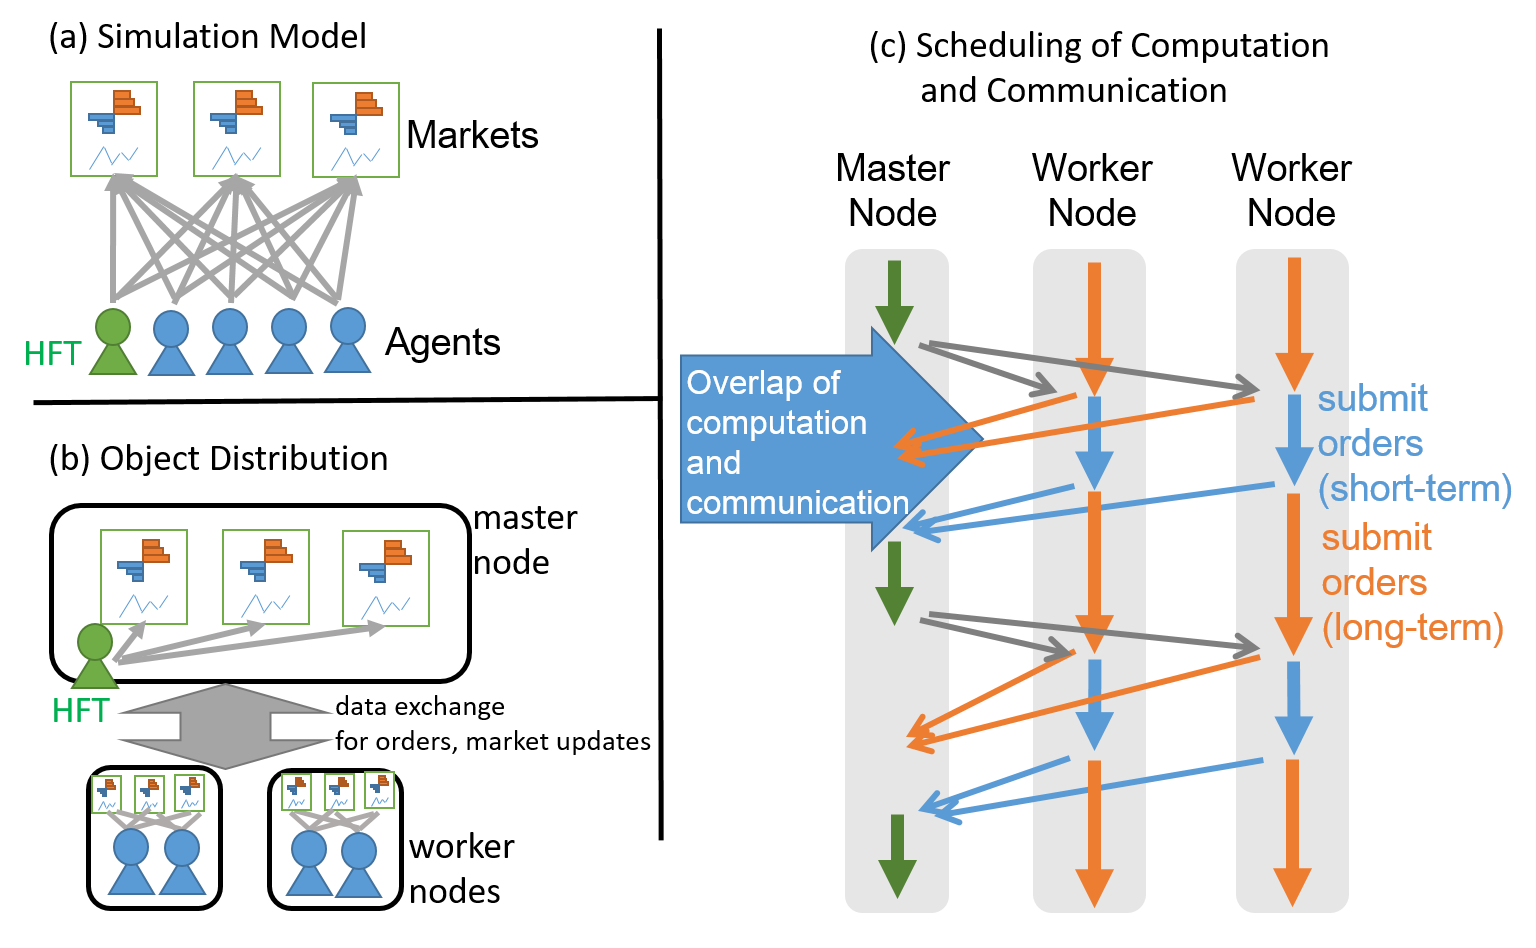
\includegraphics[width=.8\linewidth]{Figs.kamada/plham.png}
  \caption{Plham (Simulation Model and its Parallel Execution)}
  \label{fig:Figs.kamada/plham}
\end{figure}
%%++++++++++++++++++++++++++++++++++++++++++++++++++++++++++++++++++++++

Plham provides multiple runners that implement respective execution models.
To execute a parallel simulation, the users can employ a parallel runner implementing its parallel execution model that allocates agents over multiple computing nodes,
changes the scheduling frequency of agents, depending on the class of agents, and accepts delayed propagation of market information depending on the class.
In the current implementation, 
HFT agents are assigned at the master node, in which the order handling of the markets is processed,
and the computation for ordinal traders is executed at the worker nodes, as shown in Figure~\ref{fig:Figs.kamada/plham}~(b).
For large-scale simulations, nonHFT agents must be forced to make a decision by using delayed or out-of-date market information, whereas HFT agents are given access to latest or relatively up-to-date market information.

The current parallel runner allows concurrent execution of order submission and handling as shown in (c) to reduces CPU idle time at worker nodes and achieve simulation scalability.
To increase the parallelism of the simulation, the runner introduces three agent ranks: high-frequency traders, short-term traders, and long-term traders.
It then concurrently executes the order-submission stage of long-term traders and the order-handling stage of markets. 
In addition, it succeeded in overlapping communication and computation.
The scalability of the current parallel execution model was evaluated in weak-scaling to a maximum of 2048 computing nodes on the K computer~\cite{arob17plham}.
Plham is available as an open-source software under Eclipse Public License (http://github.com/crest-cassia/oacis).

To realize distributed multi-agent simulation on large scale distributed computers,
developers have to implement proper agent distribution, data transportation for agent communication, parallel execution of agent computation using multi-core CPUs, and efficient scheduling of respective components of computation and communication.
We developed a distributed collection library to easily manage
collection of object elements distributed over multiple computing nodes.
It offers methods for element relocation (communication) and data parallel processing for the elements (computation).
Our library provides a series of distributed collections, such as \texttt{DistCol[T], DistBag[T],} and
\texttt{DistMap[K,V]}, each of which manages a collection of objects that spreads over worker nodes.
Our library also prepared another type of distributed collection, \texttt{ColDist[T]}, that holds a list of objects
and allocates the cache proxies of the list at all worker nodes.
In the implementation of Plham, \texttt{ColDist} is used to manage markets and their proxies and
\texttt{DistCol} is used for agents.
Orders and contracted orders are stored into \texttt{DistBag} and \texttt{DistMap} and relocated at each calculation step.
Our library allows object transportation by using collective communication of MPI,
and the elapsed time for the communication can be reduced.
These classes also offers an asynchronous method,
\texttt{asyncEach},
that receive a function and apply it to all the local elements in the called node using thread pools.
Using these features, the overlapping of communication and computation in Plham was briefly described as shown in Figure~\ref{fig:Figs.kamada/middleware}~(a).

%%++++++++++++++++++++++++++++++++++++++++++++++++++++++++++++++++++++++
\begin{figure}
%    \centering
  \begin{minipage}{.33\textwidth}
    \begin{lstlisting}[basicstyle=\tiny, frame=single]
finish for (place in placeGroup)
 at (place) async {
  for(steps) {
    sCond = sAgents.eachAsync(..);
    if(!first) lOrders.relocate(..);
    sCond.await();
    lCond = lAgents.eachAsync(..);
    sOrders.relocate(..);
    if(master) markets.each(..); 
    markets.teamedBroadcast(..);
    contracted.relocate(..);
    lCond.await();
 }}
}
    \end{lstlisting}
  (a) Sample program of Distributed Collections
  \end{minipage}
  \hspace{4pt}
    \begin{minipage}{.3\textwidth}
      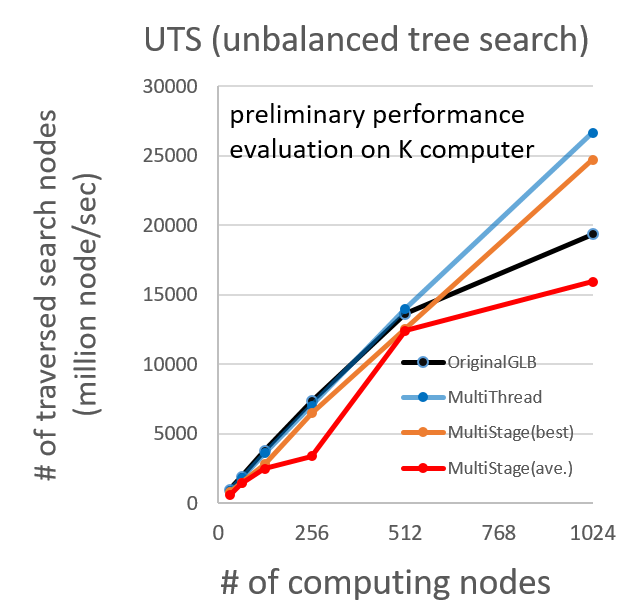
\includegraphics[width=\textwidth]{Figs.kamada/glbScale.png}
      (b) Performance evaluation of global load balancing 
    \end{minipage}
      \hspace{4pt}
        \begin{minipage}{.3\textwidth}
      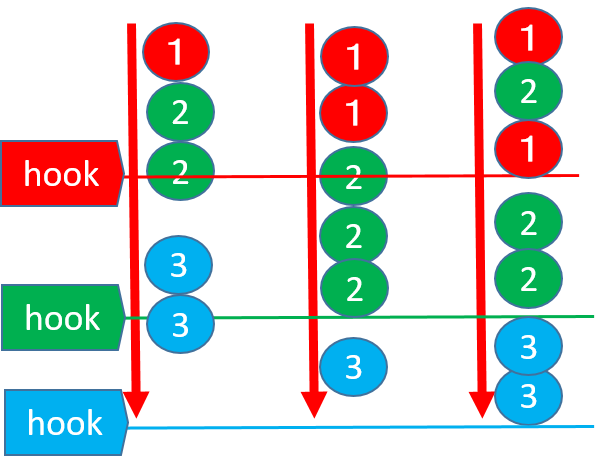
\includegraphics[width=\textwidth]{Figs.kamada/msGLB.png}
      (c) Multi-stage features for GLB
    \end{minipage}
  \caption{Parallel middleware for large-scale multi-agent simulations}
  \label{fig:Figs.kamada/middleware}
\end{figure}
%%++++++++++++++++++++++++++++++++++++++++++++++++++++++++++++++++++++++


We also conducted research on global load balancing for
 multi-agent simulation having multiple calculation steps.
Load balancing is a major concern in massively parallel computing.
X10 provides a global load balancing (GLB) library that 
shows high scalability over ten thousand CPU cores.
GLB features a lifeline-based scalable work-stealing algorithm.
Results of completed tasks are gathered by means of reduction operations.
We introduced a multithread design into GLB 
to allow efficient data sharing between CPU cores.
The multithread version showed high scalability than the original one (Figure~\ref{fig:Figs.kamada/middleware}~(b)).
In addition, we proposed a multistage mechanism for GLB to 
assign execution stages to tasks.
The system gives high priority to tasks that are assigned to earlier stages
and then proceeds with subsequent stage tasks (Figure~\ref{fig:Figs.kamada/middleware}~(c)).
When a computing node runs out of tasks at the earliest stage,
it requests tasks at the earliest stage from other nodes
and awaits responses by processing subsequent stage tasks.
When the system identifies the task termination at a certain stage,
it executes a reduction operation over nodes.
The multi-stage version has performance problems
that appear to be caused by network message scheduling or thread scheduling.
After fixing the problems,
we plan to introduce this dynamic load balancing features into our distributed collection library
to treat dynamic load imbalance of tasks.









